\subsection*{Dati di progetto}

\begin{wrapfigure}[14]{r}{0.24\textwidth}
\centering
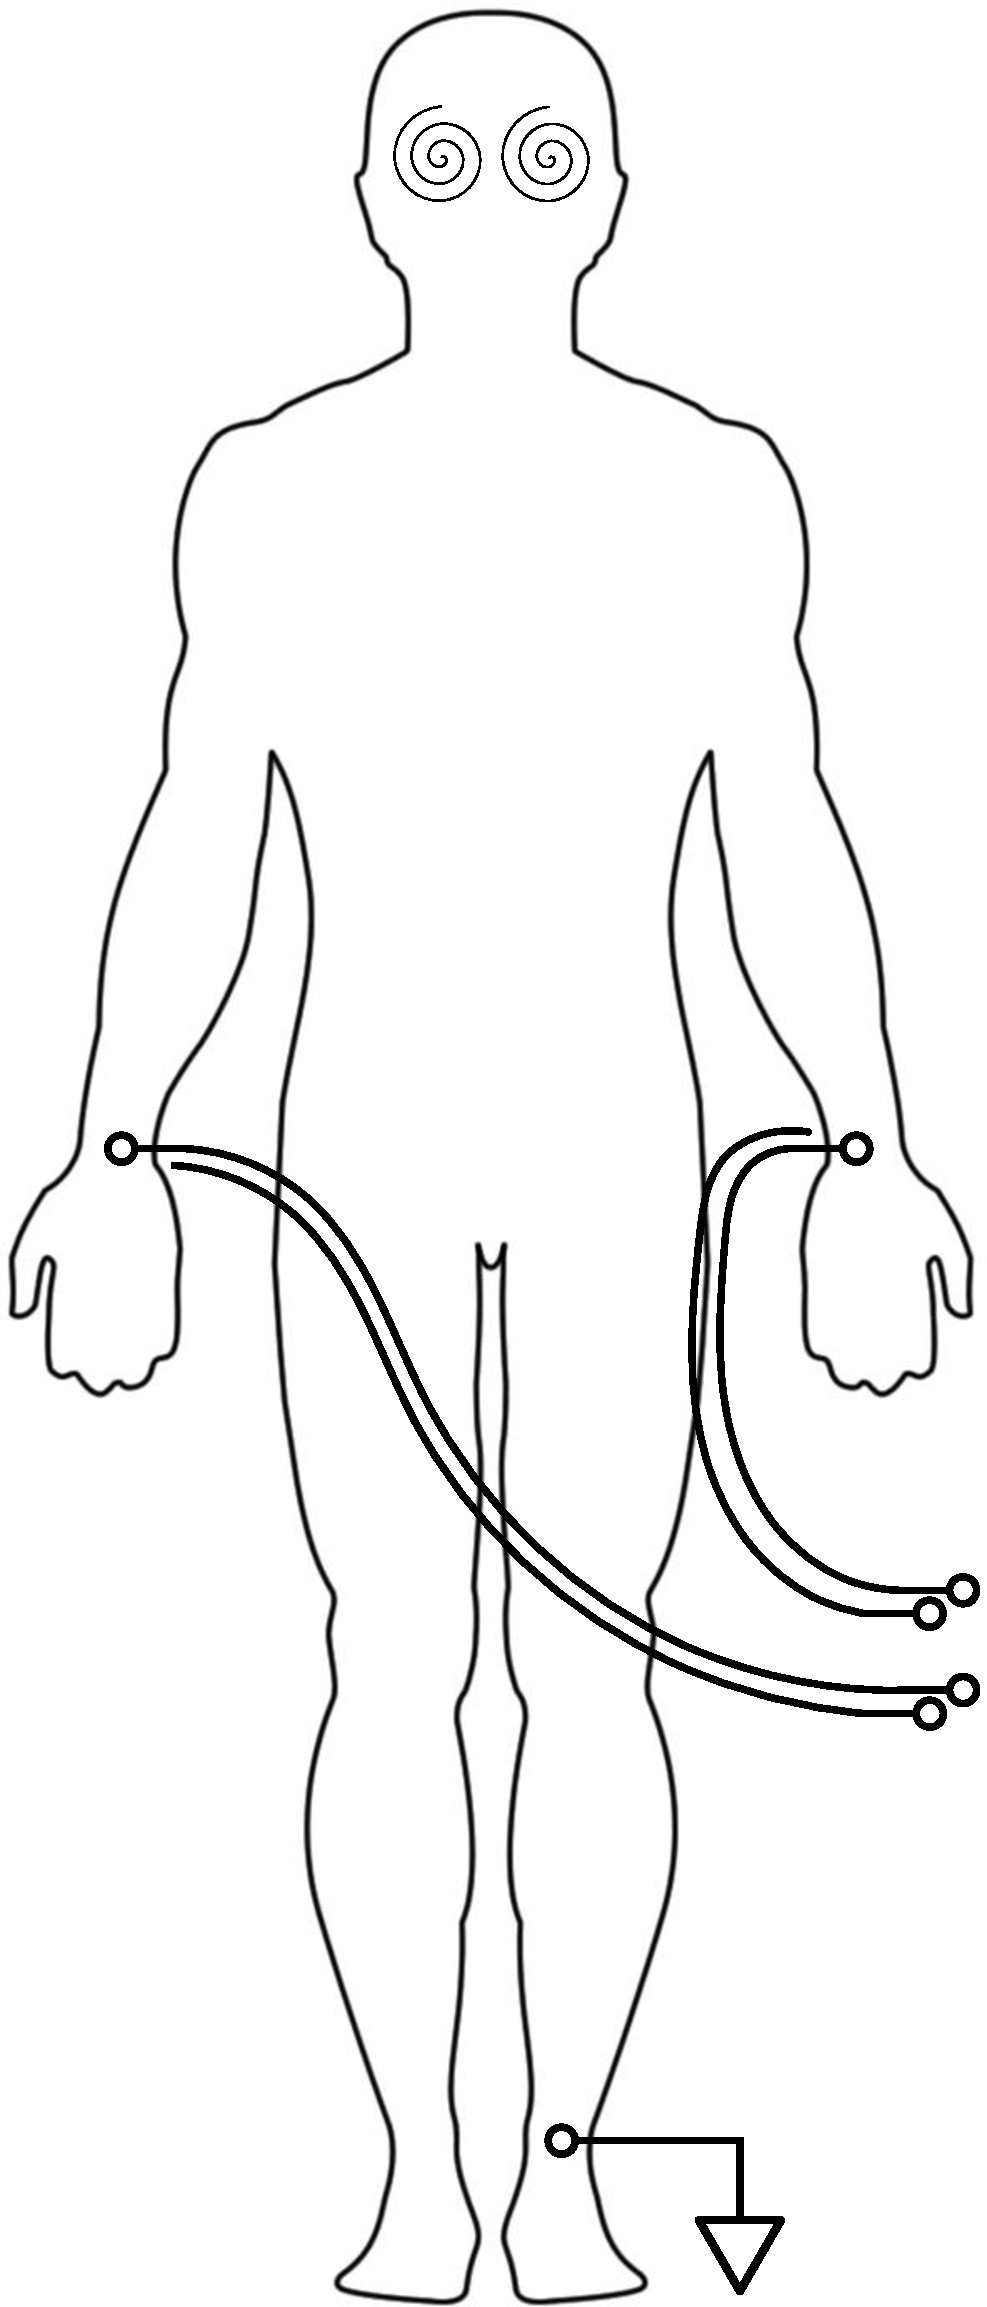
\includegraphics[width=.18\textwidth]{../E07/latex/human.pdf}
\caption{Connessioni al corpo umano}
\label{fig7:human}
\end{wrapfigure}

Per progettare un circuito che legga il segnale elettrico del nostro battito cardiaco a livello della cute, dobbiamo avere innanzitutto ben presenti alcuni punti fondamentali:
\begin{itemize} [noitemsep]
	\item Sulla superficie del corpo il segnale ECG è normalmente di circa \SI{1}{mV} (al massimo raggiunge i \SI{4}{mV}) ed ha una frequenza di circa \SI{1.25}{\Hz}.
	\item Gli elettrodi a nostra disposizione, che realizzano il collegamento tra la strumentazione e il corpo, creano un potenziale di circa \SI{700}{\mV}, quindi di circa \num{3} ordini di grandezza maggiore del segnale cardiaco.
	\item Il segnale da misurare è piccolo, quindi dobbiamo porre particolare attenzione alle fonti di rumore elettromagnetico dati da effetti capacitivi e/o induttivi. Inoltre dobbiamo evitare che i cavi e il paziente si muovano durante la misurazione.
	\item È necessario che il paziente sia isolato dal lato di elaborazione del segnale, alimentato dall'alimentatore da banco.
\end{itemize}

\subsection*{componenti}
Le parti che formeranno il circuito completo saranno:
\subsubsection{Filtro passa basso}
Il filtro passa-basso elimina i disturbi causati dalla radio-frequenza.
Con una frequenza di taglio in modo differenziale (?) di
\begin{equation*}
	\frac{1}{2 pi R ( C_d + C_c ) } = \SI{194}{\Hz}
\end{equation*}
e in modo comune di
\begin{equation*}
	\frac{1}{2 pi R C_c} = \SI{4}{\kHz}
\end{equation*}

\subsubsection{Filtro passa alto}
Il filtro passa-alto, con frequenza di taglio pari a circa \SI{3}{\Hz}, elimina la componente continua del segnale in uscita dall’amplificatore differenziale.

\subsection{Active gards}
Polarizzo la calza del cavo coassiale che connette l’elettrodo all’amplificatore ad un
potenziale pari alla tensione di modo comune.
In tal modo riduco l’effetto delle capacità parassite, e aumento la reiezione di modo
comune.
\begin{itemize}
\item il cavo che porta il segnale “vede” una differenza di potenziale molto bassa. Limito le
perdite nell’isolante
\item entrambi i cavi “vedono” lo stesso potenziale, indipendentemente dalla loro posizione sul
banco)
\end{itemize}

\subsection{Amplificatore di isolamento}
Isola galvanicamente i 2 lati del circuito: quello collegato al paziente ed alimentato a
batteria e quello di uscita ed elaborazione del segnale alimentato dall’alimentatore da
banco.
\begin{itemize}
	\item Isola fino a 1500 volt -Alimentazione da+/-4,5V a +/-18V.
	\item Possiede 2 alimentazioni separate e quindi anche due riferimenti di massa separati.
	\item Non richiede componenti esterni (tranne le capacità di disaccoppiamento)
\end{itemize}


\begin{figure}[tpc]
\centering
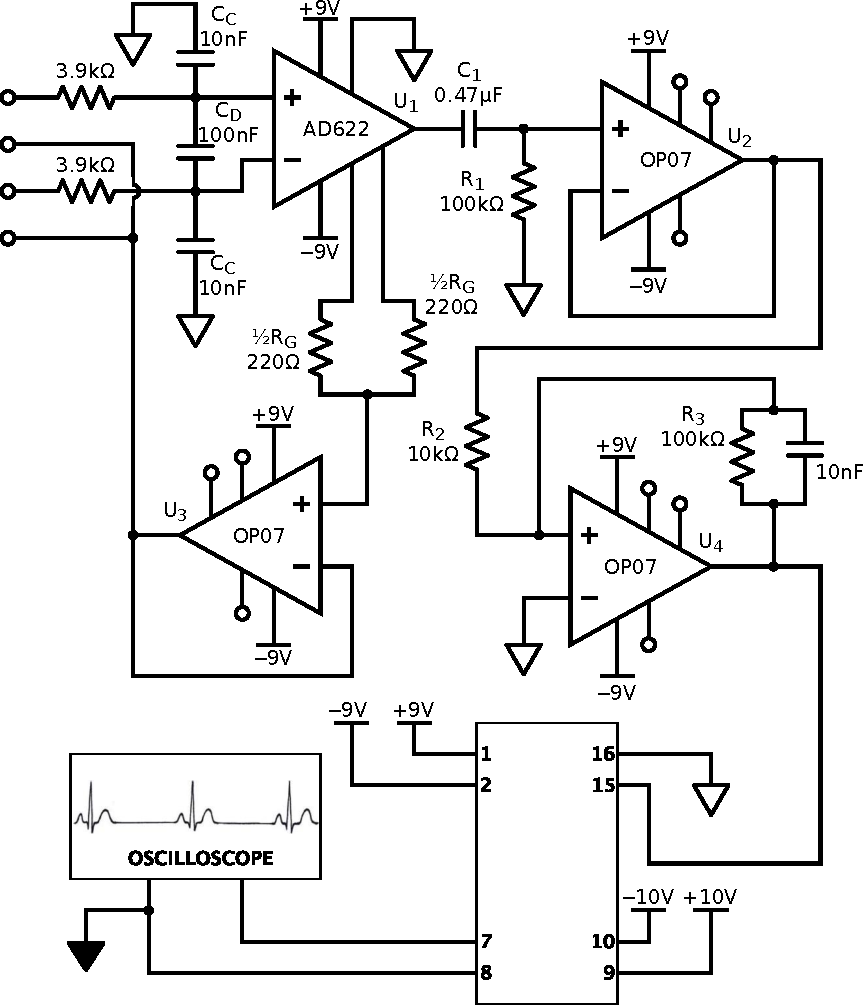
\includegraphics[width=.7\textwidth]{../E07/latex/circuito.pdf}
\caption{Schema del circuito da noi utilizzato per acquisire l'elettrocardiogramma.}
\label{fig8:compensation}
\end{figure}
